% global-visibility-commit.tex

\documentclass{standalone}
% newcommands.tex

\usepackage{amssymb, latexsym}
\usepackage{bbding} % for checkmark and xsolid
\usepackage{mathtools}

% math
\newcommand{\N}{\mathbb{N}}
\newcommand{\set}[1]{\{#1\}}
\newcommand{\bset}[1]{\big\{#1\big\}}
\newcommand{\ps}{\mathcal{P}} % for powerset
\newcommand{\emptyseq}{\emptyset} % or using <>?
\newcommand{\tuple}[1]{\langle#1\rangle} % or using (#1)?
\newcommand{\btuple}[1]{\big\langle#1\big\rangle}

\newcommand{\post}{\mathit{post}}
\newcommand{\comment}{\mathit{comment}}
\newcommand{\emptypost}{\mathit{empty}}
\newcommand{\acct}{\brown{\mathit{acct}}}

\newcommand{\yes}{\green{\Checkmark}}
\newcommand{\no}{\red{\XSolidBrush}}

\newcommand{\Key}{{\sf Key}}
\newcommand{\Val}{{\sf Val}}

\newcommand{\h}{\mathcal{H}}
%%%%%%%%%%%%%%% system models %%%%%%%%%%%%%%%
\newcommand{\E}{E}
\newcommand{\evar}{\mathit{e}}
\newcommand{\fvar}{\mathit{f}}
\newcommand{\Event}{{\sf Event}}
\newcommand{\REvent}{{\sf REvent}}
\newcommand{\WEvent}{{\sf WEvent}}
\newcommand{\HEvent}{{\sf HEvent}}
\newcommand{\op}{{\sf op}}
\newcommand{\Op}{{\sf Op}}
\newcommand{\opvar}{\mathit{op}}
\newcommand{\readevent}{{\sf R}}
\newcommand{\Read}{{\sf Read}\;}
\newcommand{\writeevent}{{\sf W}}
\newcommand{\Write}{{\sf Write}\;}
\newcommand{\WriteTx}{{\sf WriteTx}}
\newcommand{\W}{{\sf W}}
\newcommand{\R}{{\sf R}}
\newcommand{\T}{T}
%%%%%%%%%%%%%%% system models %%%%%%%%%%%%%%%

%%%%%%%%%%%%%%% axioms %%%%%%%%%%%%%%%
\renewcommand{\ae}{\mathcal{A}}
\newcommand{\axiom}{\Phi}
\newcommand{\rel}[1]{\xrightarrow{#1}}
\newcommand{\comp}{\;;\;}
\newcommand{\po}{{\sf po}}
\newcommand{\so}{\textsc{so}}
\newcommand{\rb}{\textsc{rb}}
\newcommand{\cb}{\textsc{cb}}
\newcommand{\vis}{\textsc{vis}}
\newcommand{\ar}{\textsc{ar}}
\newcommand{\hist}{\text{Hist}}
\newcommand{\intaxiom}{\textsc{Int}}
\newcommand{\extaxiom}{\textsc{Ext}}
\newcommand{\sessionaxiom}{\textsc{Session}}
\newcommand{\prefixaxiom}{\textsc{Prefix}}
\newcommand{\rbaxiom}{\textsc{ReturnBefore}}
\newcommand{\cbaxiom}{\textsc{CommitBefore}}
\newcommand{\conflict}{\bowtie}
\newcommand{\noconflictaxiom}{\textsc{NoConflict}}
\newcommand{\realtimesnapshotaxiom}{\textsc{RealtimeSnapshot}}
%%%%%%%%%%%%%%% axioms %%%%%%%%%%%%%%%

%%%%%%%%%%%%%%% consistency models %%%%%%%%%%%%%%%
\newcommand{\si}{\textsc{SI}}
\newcommand{\ansisi}{\textsc{ANSI-SI}}
\newcommand{\rtsi}{\textsc{RealtimeSI}}
\newcommand{\gsi}{\textsc{GSI}}
\newcommand{\parallelsi}{\textsc{PSI}}
\newcommand{\pcsi}{\textsc{PCSI}}
\newcommand{\strongsi}{\textsc{StrongSI}}
\newcommand{\strongsessionsi}{\textsc{SI}} % StrongSessionSI
\newcommand{\sessionsi}{\textsc{SessionSI}}
\newcommand{\nmsi}{\textsc{NMSI}}
\newcommand{\ser}{\textsc{SER}}
%%%%%%%%%%%%%%% consistency models %%%%%%%%%%%%%%%

%%%%%%%%%%%%%%% pseudo-code %%%%%%%%%%%%%%%
\newcommand{\g}{G}
\newcommand{\inducedgraph}{I}
\newcommand{\eithervar}{\mathit{either}}
\newcommand{\orvar}{\mathit{or}}
\newcommand{\reachability}{\textsc{Reachability}}
\newcommand{\reachabilityvar}{\mathit{reachability}}

\newcommand{\vertex}{\mathsf{Vertex}}
\newcommand{\edges}{\mathsf{Edge}}
\newcommand{\cons}{\mathsf{Cons}}

\newcommand{\vvar}{\mathit{v}}
\newcommand{\precvar}{\mathit{prec}}
\newcommand{\egvar}{\mathit{e}}
\newcommand{\edgevar}{\mathit{edge}}
\newcommand{\cvar}{\mathit{c}}
\newcommand{\consvar}{\mathit{cons}}

\newcommand{\BV}{\mathsf{BV}}
\newcommand{\Clause}{\mathsf{Cl}}
\newcommand{\DV}{\mathsf{DV}}
\newcommand{\formula}{\mathcal{F}}

\newcommand{\fromvar}{\mathit{from}}
\newcommand{\tovar}{\mathit{to}}
\newcommand{\typevar}{\mathit{type}}

\newcommand{\graphA}{\mathit{Dep}}
\newcommand{\graphB}{\mathit{AntiDep}}
\newcommand{\knowninducedgraph}{\mathit{KI}}
%%%%%%%%%%%%%%% pseudo-code %%%%%%%%%%%%%%%

%%%%%%%%%%%%%%% proof %%%%%%%%%%%%%%%
\newcommand{\inv}{\textsc{Inv}\;}
\newcommand{\case}{\textsc{Case}}
\newcommand{\casei}{\case\; I}
\newcommand{\caseii}{\case\; II}
%%%%%%%%%%%%%%% proof %%%%%%%%%%%%%%%

%%%%%%%%%%%%%%% checking %%%%%%%%%%%%%%%
\providecommand{\G}{}
\renewcommand{\G}{\mathcal{G}}
\renewcommand{\H}{\mathcal{H}}

\newcommand{\SO}{\textsf{SO}}
\newcommand{\WR}{\textsf{WR}}
\newcommand{\WW}{\textsf{WW}}
\newcommand{\RW}{\textsf{RW}}
%%%%%%%%%%%%%%% checking %%%%%%%%%%%%%%%

% colors
\newcommand{\red}[1]{\textcolor{red}{#1}}
\newcommand{\green}[1]{\textcolor{green}{#1}}
\newcommand{\blue}[1]{\textcolor{blue}{#1}}
\newcommand{\cyan}[1]{\textcolor{cyan}{#1}}
\newcommand{\brown}[1]{\textcolor{brown}{#1}}
\newcommand{\teal}[1]{\textcolor{teal}{#1}}
\newcommand{\purple}[1]{\textcolor{purple}{#1}}

\newcommand{\cobra}{\textsc{Cobra}}

\newcommand{\keyxvar}{\textcolor{cyan}{\mathit{x}}}
\newcommand{\keyyvar}{\textcolor{brown}{\mathit{y}}}

\usepackage{tikz}
\usetikzlibrary{calc, shapes, positioning,
  arrows.meta, decorations.pathmorphing}

\newcommand{\length}{6}

\begin{document}
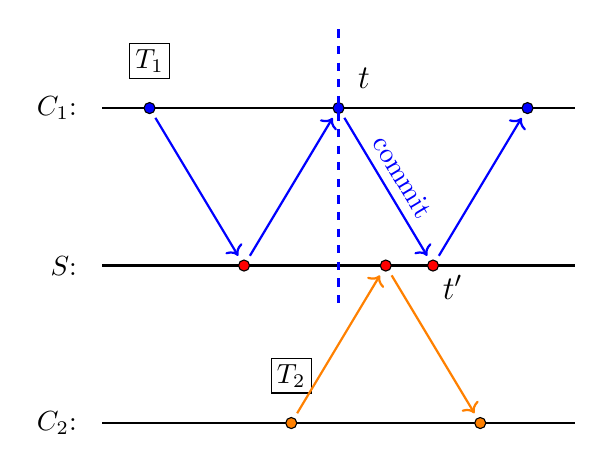
\begin{tikzpicture}[
  msg/.style = {->, thick},
  client/.style = {thick},
  txn/.style = {draw, inner sep = 2pt}]

  % c1
  \coordinate (c1-start) at (0,0);
  \coordinate (c1-end) at (\length,0);
  \draw[client] (c1-start) to (c1-end);
  \node[left = 0.20cm of c1-start] (c1) {$C_{1}$:};

  \node (c1-10) at ($(c1-start)!0.10!(c1-end)$) {};
  \node (c1-50) at ($(c1-start)!0.50!(c1-end)$) {};
  \node (c1-90) at ($(c1-start)!0.90!(c1-end)$) {};

  \node[txn, above = 0.25cm of c1-10] (t1) {$T_{1}$};

  \draw[fill=blue] (c1-10) circle [radius=2pt] node[above] {};
  \draw[fill=blue] (c1-50) circle [radius=2pt] node[above right = 5pt, font = \large] {$t$};
  \draw[fill=blue] (c1-90) circle [radius=2pt] node[above] {};

  % s
  \coordinate (s-start) at (0, -2);
  \coordinate (s-end) at (\length, -2);
  \draw[client] (s-start) to (s-end);
  \node[left = 0.20cm of s-start] (s) {$S$:};

  \node (s-30) at ($(s-start)!0.30!(s-end)$) {};
  \node (s-60) at ($(s-start)!0.60!(s-end)$) {};
  \node (s-70) at ($(s-start)!0.70!(s-end)$) {};

  \draw[fill=red] (s-30) circle [radius=2pt] node[above] {};
  \draw[fill=red] (s-60) circle [radius=2pt] node[above] {};
  \draw[fill=red] (s-70) circle [radius=2pt] node[below right = 0pt, font = \large] {$t'$};

  % c2
  \coordinate (c2-start) at (0, -4);
  \coordinate (c2-end) at (\length, -4);
  \draw[client] (c2-start) to (c2-end);
  \node[left = 0.20cm of c2-start] (c2) {$C_{2}$:};

  \node (c2-40) at ($(c2-start)!0.40!(c2-end)$) {};
  \node (c2-80) at ($(c2-start)!0.80!(c2-end)$) {};

  \node[txn, above = 0.25cm of c2-40] (t2) {$T_{2}$};

  \draw[fill=orange] (c2-40) circle [radius=2pt] node[above] {};
  \draw[fill=orange] (c2-80) circle [radius=2pt] node[above] {};

  \coordinate (above) at ($(c1-50) + (0, 1.0cm)$);
  \coordinate (below) at ($(c1-50) + (0, -2.5cm)$);
  \draw[dashed, blue, very thick] (above) to (below);

  % c1 <-> s
  \draw[msg, blue] (c1-10) to (s-30);
  \draw[msg, blue] (s-30) to (c1-50);
  \draw[msg, blue] (c1-50) to node[sloped, above] {commit} (s-70);
  \draw[msg, blue] (s-70) to (c1-90);

  % c2 <-> s
  \draw[msg, orange] (c2-40) to (s-60);
  \draw[msg, orange] (s-60) to (c2-80);
\end{tikzpicture}
\end{document}